\documentclass{aastex62}   	% use "amsart" instead of "article" for AMSLaTeX format
\usepackage{graphicx}				% Use pdf, png, jpg, or eps§ with pdflatex; use eps in DVI mode
								% TeX will automatically convert eps --> pdf in pdflatex		
\usepackage{amssymb}
\usepackage{natbib}
\usepackage{grffile}
\usepackage{textcase}
\usepackage{hyperref}
%SetFonts

%SetFonts

\begin{document}

\thispagestyle{empty}
\pagenumbering{gobble} 
\begin{description}
\item[Title]Testing Gravity Using Type Ia Supernovae Discovered by Next Generation Wide Field Imaging Survey
\item[Thematic Science Area] Cosmology and Fundamental Physics
\item[Authors] and a list of authors
\item[Lead Author Contact Information]Alex Kim; Physics Division, Lawrence Berkeley National Laboratory, 
    1 Cyclotron Road, Berkeley, CA, 94720;
1-510-486-4621;
\href{mailto:agkim@lbl.gov}{agkim@lbl.gov}
\end{description}

\clearpage
\newpage
\setcounter{page}{0}
\pagenumbering{arabic}
\setcounter{page}{1}
\title{Testing Gravity Using Type Ia Supernovae Discovered by Next Generation Wide Field Imaging Surveys}
\author[0000-0001-6315-8743]{A.~G.~Kim}
\affiliation{Physics Division, Lawrence Berkeley National Laboratory, 
    1 Cyclotron Road, Berkeley, CA, 94720}
\author{P.~Antilogus}
\affiliation{Laboratoire de Physique Nucl\'eaire et de Hautes Energies, Sorbonne Universit\'e, CNRS-IN2P3, 4 Place Jussieu, 75005 Paris, France}    
\author{S.~BenZvi}
\affiliation{Department of Physics and Astronomy, University of Rochester, Rochester, NY 14627, USA}
\author{S.~Gontcho A Gontcho}
\affiliation{Department of Physics and Astronomy, University of Rochester, Rochester, NY 14627, USA}
\author{R.~Graziani}
\affiliation{Universit\'e Clermont Auvergne, CNRS/IN2P3, Laboratoire de
Physique de Clermont, F-63000 Clermont-Ferrand, France}    
\author{C.~Harper}
\affiliation{Physics Division, Lawrence Berkeley National Laboratory, 
    1 Cyclotron Road, Berkeley, CA, 94720}
\author{C.~Howlett}
\affiliation{International Centre for Radio Astronomy Research, The University of Western Australia, Crawley, WA 6009, Australia}
\author{D.~Huterer}
\affiliation{Department of Physics, University of Michigan, 450 Church Street, Ann
Arbor, MI 48109, USA }
\author{C.~Ju}
\affiliation{Physics Division, Lawrence Berkeley National Laboratory, 
    1 Cyclotron Road, Berkeley, CA, 94720}
\author{P.-F.~Leget}
\affiliation{Laboratoire de Physique Nucl\'eaire et de Hautes Energies, Sorbonne Universit\'e, CNRS-IN2P3, 4 Place Jussieu, 75005 Paris, France}    
\author{E.~V.~Linder}
\affiliation{Physics Division, Lawrence Berkeley National Laboratory, 
    1 Cyclotron Road, Berkeley, CA, 94720}
\author{P.~McDonald}
\affiliation{Physics Division, Lawrence Berkeley National Laboratory, 
    1 Cyclotron Road, Berkeley, CA, 94720}
\author{J.~Nordin}
\affiliation{Institut fur Physik, Humboldt-Universitat zu Berlin, Newtonstr. 15, 12489 Berlin, Germany}
\author{S.~Perlmutter}
\affiliation{Physics Division, Lawrence Berkeley National Laboratory, 
    1 Cyclotron Road, Berkeley, CA, 94720}
\affiliation{Department of Physics, University of California Berkeley, 366 LeConte Hall MC 7300, Berkeley, CA, 94720-7300}
\author{N.~Regnault}
\affiliation{Laboratoire de Physique Nucl\'eaire et de Hautes Energies, Sorbonne Universit\'e, CNRS-IN2P3, 4 Place Jussieu, 75005 Paris, France}    
\author{M.~Rigault}
\affiliation{Universit\'e de Lyon, F-69622, Lyon, France; Universit\'e de Lyon
1, Villeurbanne; CNRS/IN2P3, Institut de Physique Nucl�aire de
Lyon, France}    
\author{others}

%\date{}							% Activate to display a given date or no date

\begin{abstract}
ZTF today and LSST in the upcoming decade will increase the number of identified  $z<0.3$ Type~Ia supernovae (SNe~Ia)  from the hundreds to the
hundreds of thousands.  The increase in the number density of SNe~Ia, in parallel with improvements in the standardization of
their absolute magnitudes, now make them competitive probes of the growth of structure.  The peculiar velocity power spectrum
is sensitive to $f\sigma_8$,
the product of the linear growth and amplitude of density perturbations.  Cross-correlation with synergistic galaxy surveys further constrains $f \sigma_8$ and the galaxy bias. 
Thus, in the next decade the peculiar velocities of
SNe~Ia will provide the growth of structure  in the local $z<0.3$ Universe as a powerful test of General Relativity and other models of gravity.
\end{abstract}

\section{Connection between Type Ia Supernovae Correlations and Gravity}

In the late 1990's, Type~Ia supernovae (SNe~Ia) were used as distance probes to measure the homogeneous expansion history of the Universe.  The remarkable discovery
that the expansion is accelerating  has called into question our basic understanding of the gravitational forces within the Universe.  Either it
is dominated by a ``dark energy'' that is gravitationally repulsive, or General Relativity is inadequate and needs to be replaced by a modified theory of
gravity.  It is only appropriate that in the upcoming decade, with their sheer numbers and improved distance precisions, SNe~Ia will provide measurements of the {\it inhomogeneous} motions of structures in the Universe
that will provide an unmatched test of whether dark energy or modified gravity is responsible for the accelerating expansion of the Universe.

The growth of structure depends on the expansion history of the Universe, the nature and density of its contents, and gravity. 
It is therefore a powerful probe of cosmology and dark energy.  Growth of structure can be measured from the light-emittting structures
in the Universe and from the peculiar velocities of test masses therein.
Peculiar velocities are the motions, on top of the cosmological expansion, caused by the gravitational attraction
and repulsion of density inhomogeneities in the Universe.  The peculiar velocity of an object with a known absolute magnitude
can be determined from its observer-frame magnitude and redshift. For a given background cosmology, the observed magnitude provides
an estimate of the cosmological redshift, the peculiar velocity is then the difference between the cosmological and CMB-frame redshifts.

Baryonic structures and peculiar velocities  provide a measurement of the combination $fD$.  $D$ is the ``linear growth factor'' that
gives the overall amplitude of  overdensities, and the ``linear growth rate''
$$f \equiv \frac{d\ln{D}}{d\ln{a}}$$ is how that amplitude changes with redshift.  General Relativity predicts
$f \approx \Omega_M^\gamma$ (with $D$ determined accordingly) with $\gamma=0.55$, whereas other gravity models can be similarly described
with different values of $\gamma$
\citep{2007APh....28..481L}.  
The growth of structure, through the measurement of $fD$, provides a test of General Relativity and breaks degeneracies
between gravitational and dark energy models that explain the accelerating expansion of the Universe.
Non-GR models may  also predict a change in the redshift- and scale-dependence of the growth, such observations provide additional leverage in probing gravity.
The parameter $\sigma_8$, the  standard deviation of overdensities in 8$h^{-1}$Mpc spheres, is 
commonly used in place of $D$ to normalize the
overall amplitude of  overdensities, so the standard parameterization used by the community is $f\sigma_8$.

Baryonic structures are sensitive to $f\sigma_8$ through redshift space distortions (RSD), 
which on large scales gives the combination $(b + f \mu^2)\sigma_8$ where $b$ is the bias between the tracer and dark matter
and $\mu$ gives the angular separation of Fourier modes to the line-of-sight.  Correlations between peculiar velocities are sensitive to  $f\sigma_8 (H_0 d_L)^{-1}$.
Although the velocities may be measured off of biased tracers, the tracers' dynamics are driven by all mass (including dark matter) and so are bias-free.
As
mentioned earlier, peculiar velocities are measured relative to the background cosmological expansion that
leads to the dependence on $H_0 d_L$. (Note that the combination $H_0 d_L$ is independent of $H_0$.)
Baryonic structures and peculiar velocities within the same volume are induced by the same overdensities  making their cross-correlation 
insensitive to sample variance \citep{2007PhRvL..99h1301G}: galaxy and peculiar velocity surveys provide synergistic constraints more powerful
than their naive sum.

The probative power of a specific peculiar-velocity tracer primarily depends on its number density and the precision to which its absolute magnitudes are known.
The current generation of peculiar velocity studies uses $10^3-10^5$ galaxies with Fundamental Plane and Tully-Fisher distances \citep{2008AJ....135.1738M, 2014MNRAS.445.2677S,
2016AJ....152...50T}.  These galaxies have absolute magnitude uncertainties of $\sim 0.4$~mag. 
Next generation surveys WALLABY \citep{2008ExA....22..151J} and TAIPAN \citep{2017PASA...34...47D} are designed to increase these sample sizes by an order of magnitude
over 75\% of the sky to a maximum depth of $z=0.1$.


The current sample of SNe~Ia has a low number density compared to Fundamental Plane and Tully-Fisher galaxies.
Nevertheless, their low intrinsic-magnitude uncertainties 
can provide peculiar velocities (expressed equivalently as peculiar magnitudes)
of their host galaxies \citep{2006PhRvD..73l3526H,2011ApJ...741...67D}.  Existing SN~Ia samples
have been used to test and ultimately find spatial correlations in peculiar velocities that may be attributed to the growth of structure
\citep{2008MNRAS.389L..47A,2014MNRAS.444.3926J,2015JCAP...12..033H, 2017JCAP...05..015H}.
However, the signal-to-noise is currently insufficient to perform a meaningful test of GR.

Two advances in the upcoming decade will make SNe~Ia  important probes of $f\sigma_8$.
First, the precision of SN~Ia distances can be improved.  The commonly-used empirical 2-parameter SED model yields $\sigma_M \gtrsim 0.12$~mag absolute magnitude
dispersion.  However, SNe transmit more information than just the light-curve shape and single color used in current SN models.
Recent studies indicate that with the right data, SNe absolute
magnitudes can be calibrated to $\sigma_M \lesssim 0.08$ mag \citep[see e.g.][]{2012MNRAS.425.1007B, 2015ApJ...815...58F}.  Though not yet
established, it is anticipated that such a reduction in intrinsic dispersion comes with a reduction in the magnitude bias correlated with host-galaxy properties
that is observed using current calibrations.
One such SN is worth $\gtrsim 25$ galaxies with 0.4~mag absolute magnitude uncertainty.
Secondly,  ZTF today and LSST in the upcoming decade will increase the number of identified  $z<0.3$ Type~Ia supernovae (SNe~Ia)  from the hundreds to the
hundreds of thousands, over the course of 10-years, LSST will find $\sim150,000$ $z<0.2$,  $\sim520,000$ $z<0.3$ SNe~Ia for which good light curves can be measured. This is a sample size with more galaxies at deeper redshifts than projected by WALLABY and TAIPAN.  Measurement of the velocity field using LSST-discovered
SNe~Ia has been previously quantified by \citet{2011PhRvD..83d3004B,2017JCAP...01..060O}.

The precision in  $f\sigma_8$ derived from the baseline WFD ten-year SN~Ia discoveries has been projected by \citet{2017ApJ...847..128H},
from both their RSD and peculiar velocities.
The results are summarized in Table~\ref{tab:howlett}, where a 5\% distance (0.1~mag) uncertainty is assumed for each supernova.
SNe~Ia alone can provide a $2\%$ measurement of $f\sigma_8$ at $z<0.3$ redshifts lower than where galaxy and cluster (through the
kinematic S-Z effect)
RSD measurements are sensitive.  A joint galaxy RSD and SN peculiar velocity will be even more powerful.
SNe~Ia peculiar velocities will measure $f\sigma_8$ at $z<0.3$  as well as galaxy surveys will at $z \sim 0.6$ using RSD. 
This can be compared to the current 15\% uncertainty from 6dF \citep{2017MNRAS.471..839A}, 3\% uncertainty projected
for the combined TAIPAN and WALLABY+WNSHS surveys \citep{2017MNRAS.464.2517H} for low-redshift measurements of $f\sigma_8$.
At larger $z>0.3$ redshifts DESI projects 10\% accuracies.

%{\bf Add a SN PV + DESI-like BGS column and/or a PV-only column with Cullan's code? }
% Requires the booktabs if the memoir class is not being used
\begin{table}
   \centering
   %\topcaption{Table captions are better up top} % requires the topcapt package
   \begin{tabular}{@{} lccc @{}} % Column formatting, @{} suppresses leading/trailing space
	\hline
	& RSD & RSD + PV & RSD+PV\\
	Redshift 	 & ($z$-bin) & ($z$-bin)& (cumulative)\\  \hline
      $0.00<z<0.05$   & 66.3 & 13.9 & 13.9\\
     $0.05<z<0.10$            & 24.6     &  7.3 & 6.5\\
     $0.10<z<0.15$      & 14.8  & 5.8 & 4.3\\
     $0.15<z<0.20$      & 10.6  & 5.0 & 3.3\\
      $0.20<z<0.25$     & 8.3  & 4.4 & 2.6\\
     $0.25<z<0.30$  & 6.8  &  4.0 & 2.2\\
      \hline
   \end{tabular}
   \caption{Projected percent uncertainties in $f\sigma_8$ from a 10-year LSST SN survey with 5\% distance uncertainties from
   \citet{2017ApJ...847..128H}. RSD is from clustering, and RSD~+~PV is from joint clustering and peculiar velocities.
   The cumulative column shows the effective uncertainty from combining its and all other shallower redshift bins.}
   \label{tab:howlett}
\end{table}

The projected precisions for LSST-discovered SNe~Ia have a number of interesting features. 
Despite the significant gain in volume and numbers of supernovae, the $f\sigma_8$ uncertainty in increasing redshift bins asymptotes such that 
there is little benefit in going beyond
$z=0.3$.
At $z<0.2$ the constraining power on  $f\sigma_8$ 
comes primarily from peculiar velocities
but by $z=0.3$ RSD is more important.
It turns out that for $z>0.1$, the volume is sufficiently large that the LSST sample is not yet sample variance limited.

\section{Designing a Supernova Survey to Measure $\MakeLowercase{f}\sigma_8$}
\subsection{Survey Parameters that Determine Scientific Performance}
\citet{2017ApJ...847..128H} project how well peculiar velocity surveys can measure $f\sigma_8$. 
They perform their analysis in Fourier space, 
where the Fisher information matrix of parameters $\lambda_i$ from random Gaussian field with mean zero and covariance $C(k)$ is
\begin{equation}
F_{ij} = \frac{V}{2}\int \frac{d^3k}{(2\pi)^3} \text{Tr}\left[ C^{-1} \frac{\partial C}{\partial \lambda_i} C^{-1}
\frac{\partial C}{\partial \lambda_j} \right],
\end{equation}
where the covariance for the velocity-velocity correlation
\begin{equation}
C = P_{vv}(k) + \frac{\sigma^2}{n}
\label{cov:eq}
\end{equation}
is dependent on the power spectrum, noise in the velocity measurement dominated by the intrinsic velocity dispersion $\sigma$, and the density of velocity probes
\citep{2017MNRAS.464.2517H}.  
The primary dependence on the growth of structure is through the normalization of the velocity power spectrum, such that 
\begin{equation}
 \frac{\partial P_{vv}}{\partial \lambda} = \text{constant}
\end{equation}
for the parameter choice
$\lambda=(f\sigma_8)^2$.  In the sample-variance limit, $F_{\lambda \lambda} \propto V$ whereas in the shot noise limit $F_{\lambda \lambda} \propto V n^2 \sigma^{-4}$.


The survey parameters that  enter the Fisher matrix are the volume $V$, which
in turn can be parameterized by the survey solid angle $\Omega$ and the redshift depth $z_{max}$ ; the number density of sources $n$; and the intrinsic
magnitude dispersion $\sigma_M$, where magnitude and velocity dispersions are related at low-redshift by $\sigma_{M} \approx \frac{5}{\ln{10}} \frac{1+z}{z} \sigma$.
LSST is expected to discover all $z<0.3$ SNe~Ia before maximum light in its active Wide Fast Deep (WFD) survey area.
Equating LSST discovery with having a meaningful peculiar velocity, the number density $n$ is thus a fixed parameter, which only increases with survey duration.
Thus $\Omega$, $z_{max}$, and $\sigma_M$ are left as the relevant parameters.



\begin{itemize}
\item Solid Angle $\Omega$:
The variance in $f\sigma_8$ is inversely proportional to solid angle $\Omega$.  The baseline
LSST survey covers 18,000 sq.~deg, at $-75 \lesssim \delta \lesssim15$ avoiding the Galactic plane.  Larger solid-angle coverage for $z<0.3$ SN~Ia searches, beyond
the LSST baseline, benefits peculiar-velocity science.  Complementary northern-hemisphere surveys and LSST-expanded or independent
coverage of the southern equatorial pole, could significantly increase
the sky coverage with a corresponding decrease in the variance of $f\sigma_8$.
\item Redshift Depth $z_{max}$:
For the number densities generated by LSST and the SN~Ia intrinsic magnitude dispersion, the noise is not sample-variance
limited.  We have run simulations of LSST SN surveys
and calculated the signal-to-noise (STON) of $f\sigma_8$ from the peculiar-velocity correlations. These simulations show, as seen in the left plot
of  Figure~\ref{notshot:fig}, that an increase in the number density of tracers leads to a significant improvement in STON.
It is also worth noting that sample variance is not negligible, as seen by the non-linear dependence of the  STON on $\sigma_M^2/n$. 

\begin{figure}
\centering
\includegraphics[width=0.48\textwidth]{../outcosmo/notshot.png}
\includegraphics[width=0.48\textwidth]{../outcosmo/perSN.png}
\caption{Left: STON of $f\sigma_8$ from simulated LSST SN peculiar-velocities only (no RSD).  There is a small level of scatter in the plots idue to the random
realizations made in simulating the surveys.
For several limiting redshift depths, the STON is plotted as a
function of $\sigma_M^2/n$, normalized to intrinsic magnitude dispersion $\sigma_M=0.1$~mag and 10-year LSST number densities.
Right: The effective contribution to the STON per supernova, quantified as STON divided by the root of the number of tracers.
\label{notshot:fig}}
\end{figure}

The effective contribution to the STON per supernova, quantified as STON divided by the root of the number of tracers, is higher for lower
$z_{max}$.  This is shown in the
right plot of   Figure~\ref{notshot:fig}.

A low-redshift tracer is more valuable than one at higher redshift.

\item Intrinsic Magnitude Dispersion $\sigma_M$:
A decrease in the supernova intrinsic magnitude dispersion leads to a significant improvement in  the STON of $f\sigma_8$,
as shown in Figure~\ref{notshot:fig} in parallel to our earlier discussion of the dependence of $n$.  We are not sample-variance
limited so the $\sigma^2_M/n$-term
in the Fisher matrix is important.
Survey follow-up strategy,
which determines which data are available per SN~Ia, influences the accuracy to which their distances can be determined. 
This dependence is non-trivial: the improvement between $\sigma_M=0.08$ and 0.15~mag dispersions is equivalent to a factor of 3.52
 in number density, or equivalently in survey duration. 
 
The intrinsic magnitude dispersion depends on the purity of the sample. Conservatively, we consider
a pure SN~Ia sample obtained through
spectroscopic classification; the requisite follow-up resources needed for complete $z<0.3$ coverage is conceivable. 
The feasibility of using photometric classification is an important subject of research
that can have implications for survey planning, particularly in extending the redshift range.
\end{itemize}

\subsection{Designing an SN~Ia Peculiar Velocity Survey}
There are different options to consider in the design of a SN~Ia peculiar velocity survey, though at this point it is difficult to assess which is optimal
or most cost effective.  While there are a variety
of recently identified indicators of SN~Ia diversity that improve upon the 2-parameter model (SALT2) currently used to determine distances, 
there is not yet an umbrella model that simultaneously captures all indicators, their correlations, and characterizes the model residuals.
Here we  make several general conclusions
based upon the above findings, while noting that 
constructing such a model is a parallel
endeavor that will benefit peculiar-velocity  and other SN~Ia science. 

\begin{itemize}
\item Spectroscopic transient classification:  SNe~Ia are defined through the absence of Hydrogen and the presence of the 6150~\AA~Silicon P-Cygni feature.
\item Spectroscopic redshifts:  Peculiar velocities are extracted directly from redshift measurements.  Redshift uncertainties of $>0.5$\% contribute significantly
to the error budget.  We thus conclude that there is the need for spectroscopic $R>200$ host-galaxy redshifts.  In most cases this redshift will be
available in the classification spectrum.  Planned bright-galaxy redshift surveys can also observe a significant fraction of nearby SN hosts.
\item Role of LSST:
LSST can be taken to be a SN~Ia discovery and distance machine, or a discovery machine only.   The nominal cadence  
 produces sparse per-band light curves, which limits the intrinsic magnitude dispersion possible with LSST data alone to $\sigma_M \approx 0.15$~mag.
The wide-field of LSST is
 well suited for discoveries over a larger area of sky, but does not provide significant multiplex advantage for the low surface-density of active
$z<0.3$ SNe~Ia.  LSST is suited for maximizing $\Omega$ while other (cheaper) resources that supplement LSST photometry can improve $\sigma_M$.
The ultimate WFD observing strategy determines how well $\sigma_8$ can be determined with LSST data alone, and the amount of external resources needed  (if any) to
reach a targeted $\sigma_M$.
\item Follow-up resources to determine per-SN distances:
Supplemental non-LSST follow-up data in the form of improved temporal light-curve sampling (accurate rise and decline times), 
expanded (UV, NIR) wavelength coverage, and spectral features
can access high-fidelity SN~Ia models with lower intrinsic magnitude dispersion and residual systematic bias.
For example, infrared data \citep{2012MNRAS.425.1007B} or spectrophotometry at peak brightness
 \citep{2015ApJ...815...58F} are projected to give $\sigma_M \lesssim 0.08$~mag.

Scientific leverage dictates that low-redshift sources are most valuable.
This aligns with observational considerations, for which closer and hence brighter objects require more modest follow-up resources.
Therefore, $z_{max}$ depends on the follow-up program as the redshift where complete follow-up saturates resources.

A follow-up survey with $z_{max}=0.2$ would have $\sim 150,000$ targets over 10 years.  These sources will be observed when
brighter than $r \sim 20.5$~mag and so will be accessible to 2--4m-class telescopes.  
\end{itemize}


\section{Conclusions}
SNe~Ia are already powerful probes of the homogeneous cosmological expansion of the Universe.  In the next decade.
high-cadence, wide-field imaging surveys, together with improved precision in their distance determinations, will make SNe~Ia powerful probes
of the gravity induced-motion caused by the inhomogeneous Universe.  SNe~Ia peculiar velocities at $z<0.3$ will measure $f \sigma_8$ significantly better
than galaxy surveys, at lower redshifts that provide better leverage to test gravity models.
While imaging surveys will provide a steady stream of SNe~Ia, a coordinated plan of follow-up is required to take advantage of
their probative power.  The resources necessary to follow hundreds of thousands of SNe depend on specific follow-up choices, and 
access to those resources will define the redshift limits of the survey.  Fortunately, the lowest-redshift, and hence brightest, supernovae
are of the highest interest, so that a modest suite of $\sim 5$ 2--4m telescopes should be capable of providing leading measurements of
$f\sigma_8$ at $z\sim 0.1$.


%
%
%\appendix
%\section{Reanalysis in Configuration Space}
%
%This Appendix describes a new analysis used to project precisions on $f\sigma_8$ using peculiar velocities derived from SNe~Ia.
%This analysis may or may not be useful for the Decadal Survey White Paper, but will be helpful for LSST planning.
%While there have been a number of articles on the subject,
%our analysis brings a higher level of fidelity than sought previously.  We simulate SNe~Ia hosted by galaxies in a mock galaxy
%catalog. The numbers of SNe are sufficiently small to allow fast evaluations of the likelihood, which enable the determination of parameter
%posteriors using MCMC on reasonable computing timescales.   We can use our machinery to 
%compare different survey parameters, such as redshift depth, total numbers of supernovae, non-uniform spatial density,
%solid angle/survey geometry, and SN~Ia intrinsic magnitude dispersion.
%Adding the cross-correlation between galaxy-count and peculiar-velocity surveys is active work, so we can
%quantify the suppression of sample variance achieved when considering matter-densities and velocities 
%within the same volume \citep{2007PhRvL..99h1301G}.
%
%\section{Simulated Data}
%The cosmoDC2 (v1.0) covering 706 sq.~deg is used\footnote{We previously used
%Buzzard (v1.6) galaxy catalog is used, but it was found to give peculiar velocities inconsistent with general relativity.  As we will see,
%cosmoDC2 (v1.0) is consistent with GR. }. 
%The catalog is based on a Flat $\Lambda$CDM model with $H_0=71$~km~s$^{-1}$,  $\Omega_M=0.265$, $\Omega_B=0.0448$, and
%$\Omega_\nu=0$.
%Each galaxy has its cosmological redshift, the $x$-, $y$-, $z$-components of its peculiar velocity from which
%the radial peculiar velocity is determined, and its
%star formation rate and stellar mass from which the
%supernova rate of each host is determined using 
%\citet{2012ApJ...755...61S}.   This host-based rate
%underestimates the expected discovery based on the volumetric
%rate of \citet{2010ApJ...713.1026D}.  The volumetric rate is more robust, so  we boost the SN production
%by a factor 2.4 to get the 10-year volumetric rate expectation. The total number of simulated SNe 
%is greater than the total number of possibly useful supernova discoveries, since most fields cannot be continuously monitored throughout the year
%from most ground-based observatories.
%
%
%Each supernova is assigned a magnitude based on the distance modulus of its cosmological
%redshift plus a random term drawn from a Normal distribution $\sigma_M$, which for simplicity is the same for all supernovae and captures both
%intrinsic magnitude dispersion and measurement uncertainty.  No other corrections are applied to the observed magnitude.  Dipole effects of the heliocentric
%motion with respect to the CMB and of the galaxies with respect to the CMB  are ignored: referring to
%\citet{2011ApJ...741...67D}, the effects in Eq.~18 are not included.  Including these effects are straightforward but is computationally expensive
%and does not affect our conclusions.
%
%We consider a maximum redshift of $z=0.2$ because over ten years the noise is not sample-variance dominated, meaning that the differential improvement
%in the precision of
%$f\sigma_8$ due to a lower-redshift supernova is greater than that due to a high-redshift supernova.  Following all LSST SNe~Ia below this redshift 
%would likely saturate available follow-up resources.
%
%
%\section{Analysis}
%The analysis is  almost identical to that of \citet{2015JCAP...12..033H, 2017JCAP...05..015H}, except as noted later.  
%The peculiar magnitude is given by 
%\begin{equation}
%\delta_m=(m - M) - \mu(z;H_0, \Omega_M, \Omega_\Lambda).
%\label{data:eqn}
%\end{equation}  We introduce one free parameter 
%$\mathcal{M} = M - 5\log{H_0} + \text{const}$ and do not consider the other cosmological parameters, whose effects are relatively weak at low-redshift.
%
%
%The peculiar magnitude correlation
%function $\xi_{\delta m \delta m}$ \citep{2011ApJ...741...67D,2015JCAP...12..033H} expected from General Relativity acting on the CMB
%matter density power spectrum is calculated using CAMB \citep{Lewis:2002ah}  assuming the same
%cosmological parameters used for the cosmoDC2 catalog.  Our model for the data covariance
%is
%\begin{equation}
%C_{ij} = A\xi_{\delta m \delta m}(\mathbf{r_i},\mathbf{r_j}) + \frac{\sigma_M^2}{N_i} \delta_{ij} + \sigma^2_{NL}(z_i;\sigma_{v})\delta_{ij},
%\label{cov:eqn}
%\end{equation}
%where $N_i$ is the number of SNe~Ia in galaxy $i$ and $\sigma_M$ is the intrinsic SN magnitude dispersion.
%The model is used to test General Relativity through deviations from $A=1$ but is not sensitive to deviations
%from the linearized GR expectation of the shape of the power spectrum 
%$\xi$.
%Nevertheless, for
%convenience we say that our model gives $f\sigma_8 = A (f\sigma_8)^{GR}$, where $(f\sigma_8)^{GR}$ is the expectation
%from General Relativity. 
%The final term includes extra magnitude dispersion produced by non-linear effects on velocity, parameterized with $\sigma_{v}$, such that
%\begin{equation}
%\sigma_{NL} = \frac{5}{\ln{10}} \frac{1+\bar{z}}{\bar{z}} \sigma_v,
%\end{equation}
%where $\bar{z}$ is the cosmological redshift of the host galaxy.
%We note that the CAMB calculation of $\xi$ includes non-linear corrections, which actually may be a bad thing for peculiar velocities \citep{2015MNRAS.454.3920H}. 
%Such subtleties are unimportant as \citet{2015JCAP...12..033H} find that their results are insensitive to whether non-linear corrections are or are not included.
%
%For all analyses we remove supernovae below observed $z_{min}=0.01$ in order to
%reduce errors made in the first-order transformation between velocity and
%magnitude.  This cut removes a  small volume relative to the full survey.
%
%The posterior of the parameters is sampled using emcee.  The likelihood is the Normal distribution with the data in Eq.~\ref{data:eqn} and
%covariance matrix in Eq.~\ref{cov:eqn}.
%The priors are positive and flat for $A$, flat for $M$, positive Cauchy(0.08, 0.5) for $\sigma_M$, and  positive Cauchy(0, 600 km~s$^{-1}$) for $\sigma_{v}$.
%
%Direct tests of non-GR models for which Poisson's equation or the linear approximation
%does not apply requires a model-dependent $\xi$.  We defer the analysis of such higher-fidelity models to later work. 
%
%\section{Results of Subsets}
%
%The  ston in $f\sigma_8$ is calculated for different subsamples of the simulated data.
%For each subsample  the mean  and standard deviation, $(\bar{A}, \sigma_A$) of the amplitude parameter is
%determined.  The ston in $f\sigma_8$ for the subsample is thus  $\bar{A} \sigma^{-1}_A$, and that for a 18,000 sq.~deg. survey  is approximated by
%$\sqrt{18000/760}\bar{A}\sigma^{-1}_A$.  The effective constraining power of a single supernova in the subset is chracterized by 
% $\bar{A} \sigma^{-1}_A N_{gal}^{-0.5}$.
%
%Different parameters describing the input simulated data define the subsamples, 
%which are used to explore the range of possible survey strategies.   The varied parameters are the redshift range, $z_{max}$, intrinsic
%magnitude dispersion, $\sigma_M$, and SN number density, $n = \phi n_{10}$, where $ n_{10}$ is the  10-year total number density.  In general a given point
%of sky is not monitored over the full year.  
%The fit posterior for one representative subsample, with input  $z_{max}=0.2$, $\sigma_M=0.08$, $\phi=0.65$, is shown in Figure~\ref{zmax:fig}.
%For all subsamples, there is no evidence for non-convergence of the MCMC chains.  The parameter $\sigma_v$, not included in  \citet{2015JCAP...12..033H, 2017JCAP...05..015H},
%is found to be consistent with zero, poorly constrained, and very weakly correlated with $A$.  Table~\ref{tab:subsets} gives the results for the different subsamples.
%
%\begin{figure}
%\centering
%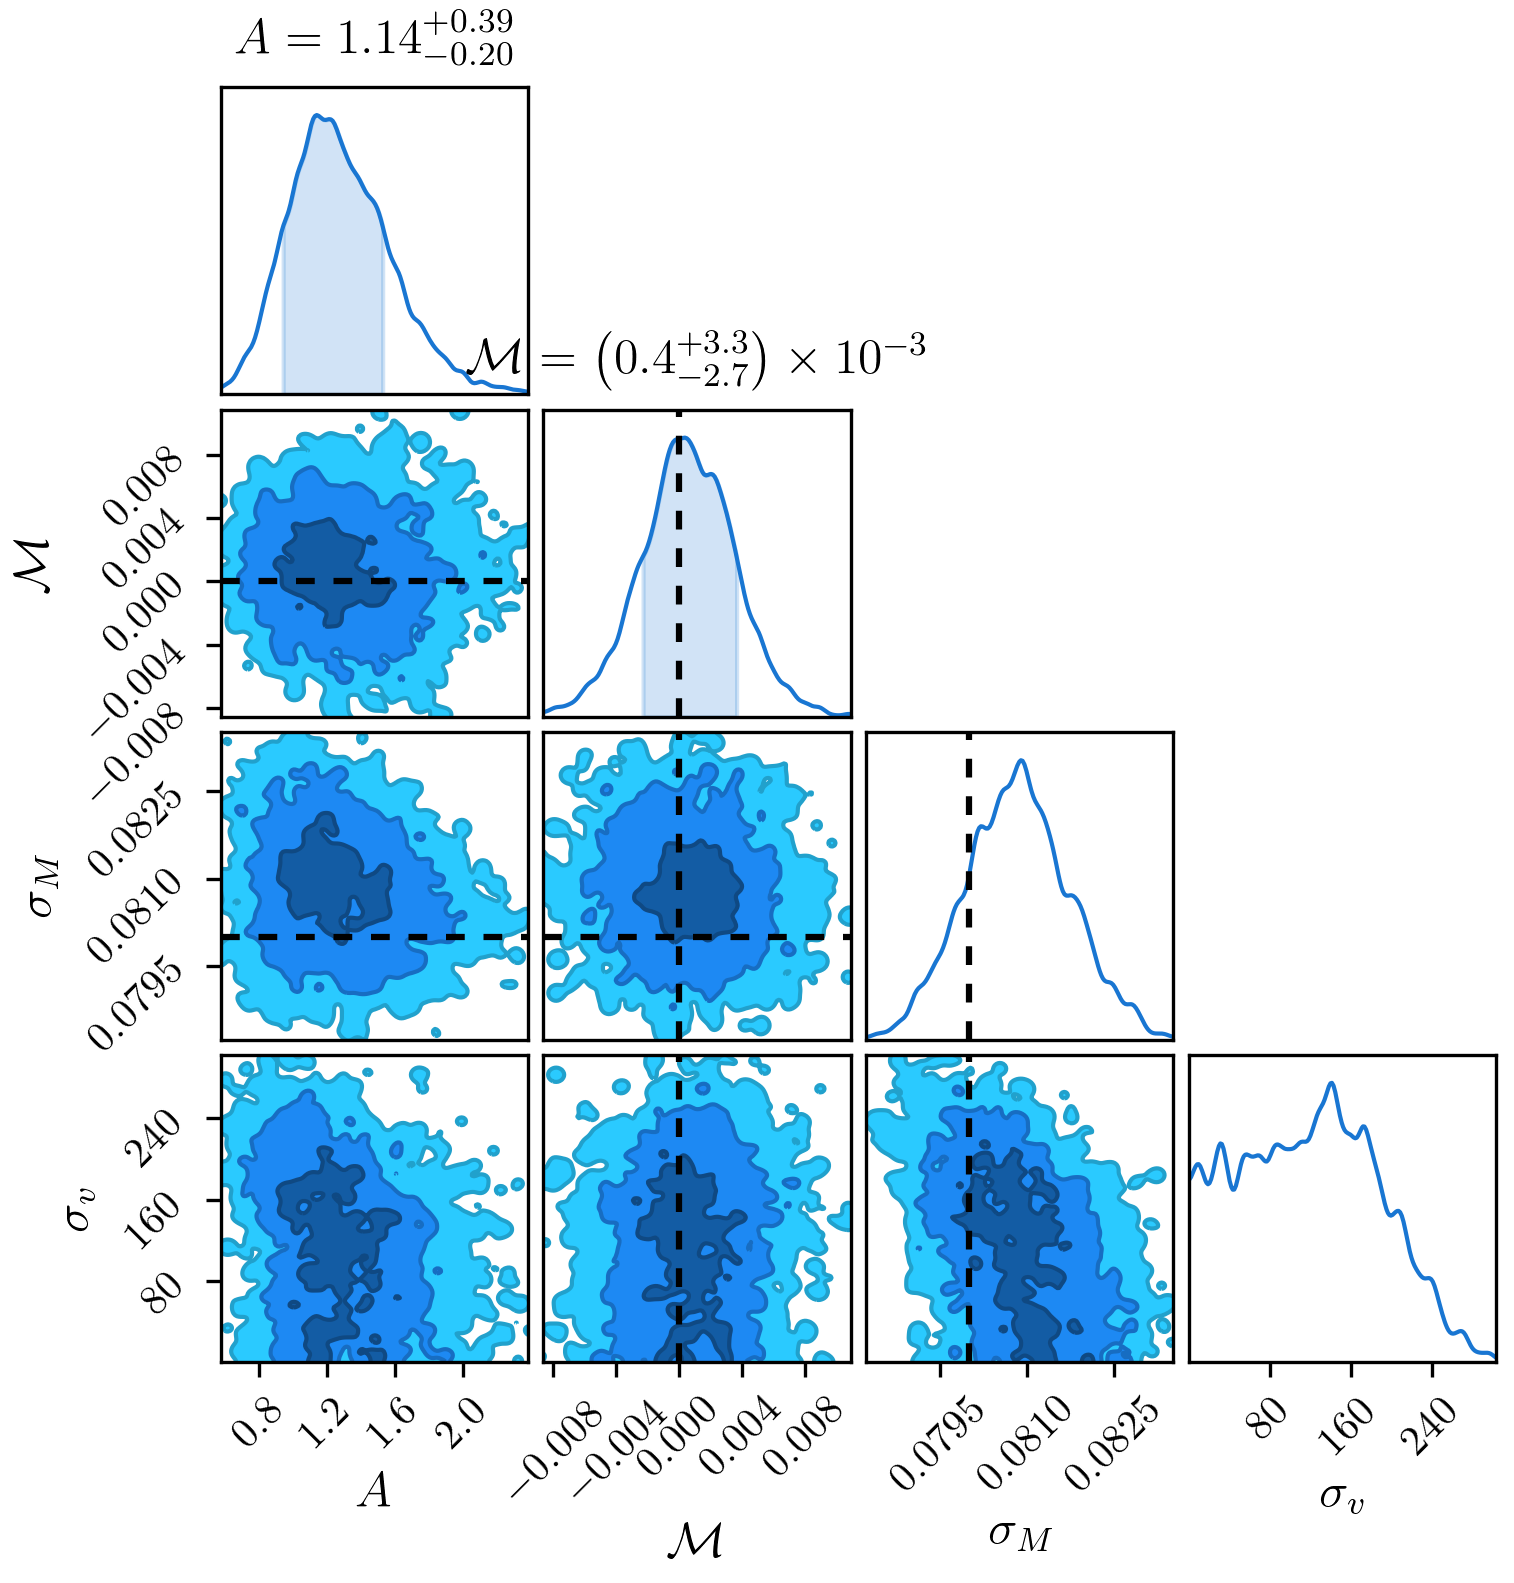
\includegraphics[width=0.5\textwidth]{../outcosmo/pvlist.0.08.1234.0.65.0.2.pkl.png}
%\caption{Confidence regions for the model parameters.  $A=(f\sigma_8)/(f\sigma_8)_{GR}$, $\mathcal{M}$ is the supernova
%absolute magnitude, $\sigma_M$ is the magnitude dispersion, and $\sigma_v$ is the non-linear contribution
%to peculiar velocity.  This result is for the subset $z_{max}=0.2$, $\sigma_M=0.08$, $\phi=0.65$.  The dotted lines represent the inputs of the supernova
%part of the simulation.
%\label{zmax:fig}}
%\end{figure}
%
%\begin{table}
%   \centering
%   %\topcaption{Table captions are better up top} % requires the topcapt package
%   \begin{tabular}{|ccc|cc|} % Column formatting, @{} suppresses leading/trailing space
%   \hline
%$z_{max}$ & $\phi$ & $\sigma_{M}$  &  STON $f\sigma_8$ & STON per SN \\
%\hline
%0.07 & 0.65 & 0.08  & 25.795 &   0.27 \\
%0.07 & 1.00 & 0.08  & 31.163 &   0.27 \\
%0.07 & 1.00 & 0.10  & 25.421 &   0.22 \\
%0.07 & 1.00 & 0.12  & 22.173 &   0.19 \\
%0.07 & 1.00 & 0.15  & 18.831 &   0.16 \\
%0.10 & 0.30 & 0.08  & 23.784 &   0.24 \\
%0.10 & 0.50 & 0.08  & 23.501 &   0.18 \\
%0.10 & 0.65 & 0.08  & 24.994 &   0.17 \\
%0.10 & 0.65 & 0.10  & 20.866 &   0.15 \\
%0.10 & 0.65 & 0.12  & 18.778 &   0.13 \\
%0.10 & 1.00 & 0.08  & 31.704 &   0.18 \\
%0.10 & 1.00 & 0.10  & 25.687 &   0.15 \\
%0.10 & 1.00 & 0.12  & 22.982 &   0.13 \\
%0.15 & 0.30 & 0.08  & 24.799 &   0.15 \\
%0.15 & 0.30 & 0.12  & 19.527 &   0.12 \\
%0.15 & 0.50 & 0.08  & 29.550 &   0.14 \\
%0.15 & 0.65 & 0.08  & 33.921 &   0.14 \\
%0.15 & 0.65 & 0.10  & 28.655 &   0.12 \\
%0.15 & 0.65 & 0.12  & 24.111 &   0.10 \\
%0.15 & 1.00 & 0.08  & 40.158 &   0.13 \\
%0.20 & 0.20 & 0.08  & 26.487 &   0.12 \\
%0.20 & 0.30 & 0.08  & 29.828 &   0.11 \\
%0.20 & 0.30 & 0.10  & 24.019 &   0.09 \\
%0.20 & 0.30 & 0.12  & 19.181 &   0.07 \\
%0.20 & 0.50 & 0.08  & 36.680 &   0.11 \\
%0.20 & 0.65 & 0.08  & 41.591 &   0.11 \\
%0.20 & 0.65 & 0.10  & 35.196 &   0.09 \\
%0.20 & 0.65 & 0.12  & 27.987 &   0.07 \\
%0.20 & 1.00 & 0.08  & 48.368 &   0.10 \\
%0.20 & 1.00 & 0.10  & 40.835 &   0.08 \\
%0.20 & 1.00 & 0.12  & 37.875 &   0.08 \\
%    \hline
%   \end{tabular}
%   \caption{ston in $A$ or equivalently $f\sigma_8$ for surveys parameterized by the maximum redshift $z_{max}$,
%   the fraction of total supernovae in 10 years ``fraction'', intrinsic magnitude dispersion $\sigma_{SN}$.  The number of galaxies
%   $N_{gal}$, the signal $\bar{A}$ and its uncertainty $\sigma_A$ are for the cosmoDC2 (v1.0) 760 sq.~deg. volume only.
%   The uncertainty ``per'' supernova is given by  $\sigma_A N_{gal}^{-0.5}$.  The ston, scaled to an LSST solid angle, is given as 
%    $\bar{A} \sigma_A^{-1} (18000/760)^{0.5}$.
%   \label{tab:subsets}}
%\end{table}
%
%In Fourier space, the data covariance is a combination of sample and shot noise (Eq.~\ref{cov:eq}).
%In Figure~\ref{scaling:fig} the effective LSST ston is plotted as a function of input $n \sigma^{-2}_M$ for different $z_{max}$.
%For all cases, the ston improves with larger $n \sigma^{-2}_M$ showing that the sample-variance limit has not been reached,
%though the shallowing of the slopes for shallower surveys shows that it does contribute non-negligibly.
%The fact that the ston is not constant indicates that not of the subsamples is sample-variance limited, though its non-linearity
%indicates that it is non-negligible.
%
%
%\begin{figure}
%\centering
%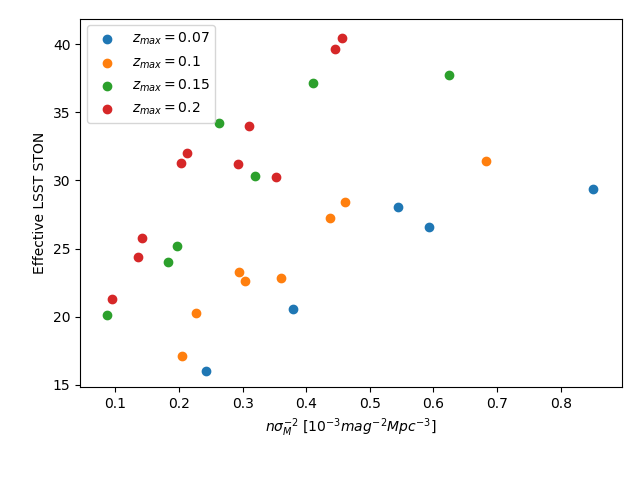
\includegraphics[width=0.5\textwidth]{../outcosmo/fracsnsig2_.png}
%%\includegraphics[width=0.5\textwidth]{../outcosmo/zmax_.png}
%\caption{ Effective LSST ston as a function of input  $n \sigma^{-2}_M$.  The points are color-coded for different $z_{max}$.
%\label{scaling:fig}}
%\end{figure}
%
%A SN peculiar survey benefits from greater redshift depth $z_{max}$ due to the increase in volume and numbers of supernovae.  However,  for fixed magnitude uncertainty
%peculiar-velocity uncertainties increase with redshift and the follow-up of fainter distant SNe requires more resources. 
%Table~\ref{tab:subsets}
%shows that the effective worth of each supernova ($\sigma_A N_{gal}^{-0.5}$) diminishes with increasing survey depth.
%The table also shows that for $\sigma_M=0.08$~mag, the subsample with $z_{max}=0.1$ with 1294 supernovae yields a ston of 15.96, whereas
%a sample with $z_{max}=0.2$ with 2021 supernovae has a lower ston of 13.61.  Within the range of surveys considered, a lower-redshift supernova
%is more valuable than one at high redshift.  For both scientific and resource reasons, it is best to devote resources to the lowest possible redshifts.
%
%
%$\phi \sim 0.65$ is an effective number density of discovered supernovae with light-curve coverage observed in 10 years
%

\bibliographystyle{aasjournal}
\bibliography{/Users/akim/Documents/alex}

\end{document}  